\documentclass[conference,onecolumn]{IEEEtran}
\IEEEoverridecommandlockouts
% The preceding line is only needed to identify funding in the first footnote. If that is unneeded, please comment it out.
\usepackage{cite}
\usepackage{amsmath,amssymb,amsfonts}
\usepackage{algorithmic}
\usepackage{graphicx}
\usepackage{hyperref}
\usepackage{textcomp}
\usepackage{xcolor}
\def\BibTeX{{\rm B\kern-.05em{\sc i\kern-.025em b}\kern-.08em
    T\kern-.1667em\lower.7ex\hbox{E}\kern-.125emX}}
\begin{document}

\title{Project Management System}

\author{\IEEEauthorblockN{Arpit Vaghela}
  \IEEEauthorblockA{\textit{Ahmedabad University}\\
    \href{mailto:arpitsinh.v@ahduni.edu.in}{arpitsinh.v@ahduni.edu.in}\\
    AU1841034}
  \and
  \IEEEauthorblockN{Kaushal Patil}
  \IEEEauthorblockA{\textit{Ahmedabad University}\\
    \href{mailto:kaushal.p@ahduni.edu.in}{kaushal.p@ahduni.edu.in}\\
    AU1841040}
  \and
  \IEEEauthorblockN{Dhruvil Dave}
  \IEEEauthorblockA{\textit{Ahmedabad University}\\
    \href{mailto:dhruvil.d@ahduni.edu.in}{dhruvil.d@ahduni.edu.in}\\
    AU1841003}
}

\maketitle

\begin{abstract}
  This is a project management system written using \href{https://reactjs.org/}{React.js} for frontend, \href{https://flask.palletsprojects.com/en/1.1.x/}{Flask} and \href{https://graphql.org/}{GraphQL} for backend and \href{https://www.postgresql.org/}{PostgreSQL} as database. This project was made as a part of subjects Database Management Systems (CSE250) and Database Management Systems Lab (CSE251). This project allows users to have an entire project management functionalities like creating projects, adding members, adding tasks, adding and managing boards, notes etc. in one place like the one provided by popular platforms like GitHub, GitLab etc.

  To run the project, do the following steps:
\end{abstract}

\newpage
\section{ER Diagram}
\begin{center}
  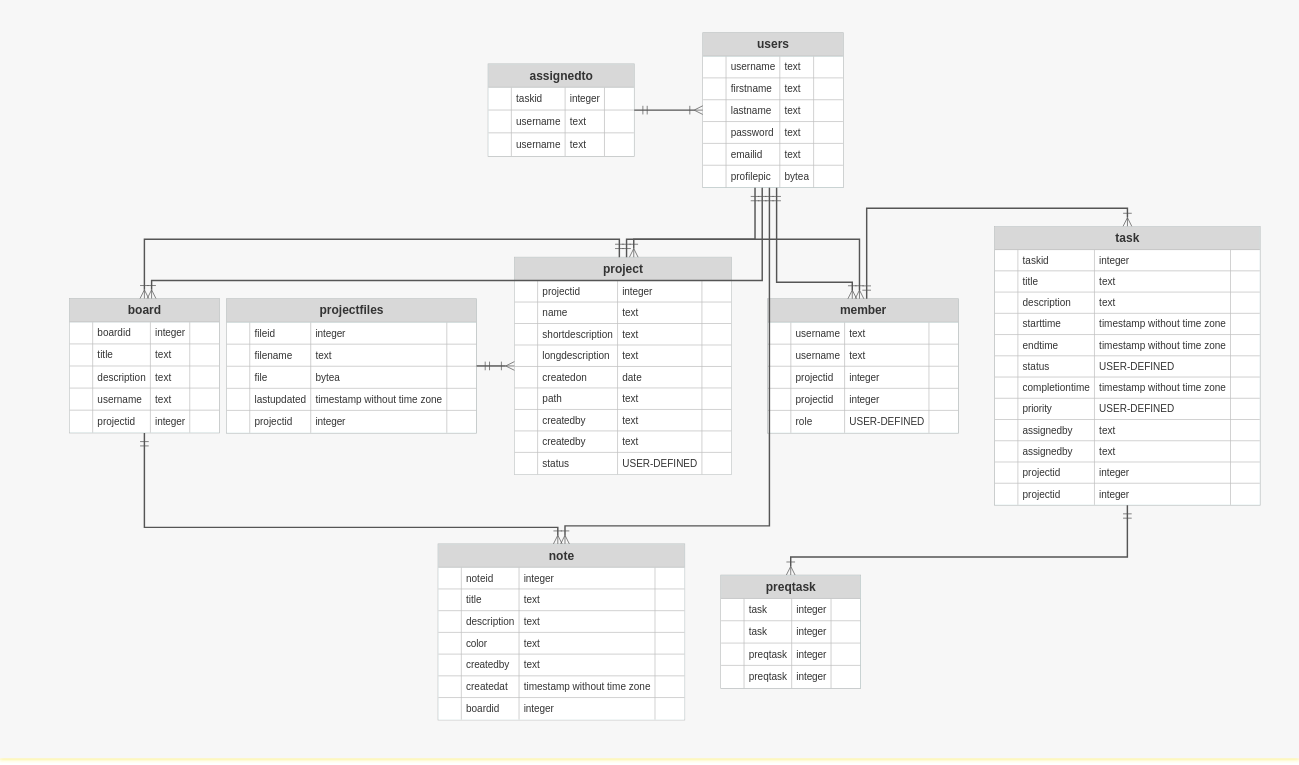
\includegraphics[scale=0.3]{ERD.png}
\end{center}

\section{Table Design}
\begin{table}[htbp]
  \caption{Users}
  \begin{center}
    \begin{tabular}{|c|c|c|c|}
      \hline
      \textbf{Column} & \textbf{Type} & \textbf{Nullable} & \textbf{Default}\\
      \hline
      username & text & not null & \\
      firstname & text & not null & \\
      lastname & text & not null & \\
      password & text & not null & \\
      emailid & text & not null & \\
      profilepic & byte array & & \\
      \hline
    \end{tabular}
    \begin{enumerate}
    \item Indexes:
      \begin{enumerate}
      \item PRIMARY KEY (username)
      \item UNIQUE CONSTRAINT (emailid)
      \end{enumerate}
    \item Check Constraints:
      \begin{enumerate}
      \item emailid
      \item firstname
      \item lastname
      \item username
      \end{enumerate}
    \item Referenced by:
      \begin{enumerate}
      \item assignedto \ref{assignedto}
      \item board \ref{board}
      \item member \ref{member}
      \item note \ref{note}
      \item project \ref{project}
      \end{enumerate}
    \item Triggers:
      \begin{enumerate}
      \item add\_board AFTER INSERT ON users FOR EACH ROW EXECUTE FUNCTION add\_board()
      \item create\_hash BEFORE INSERT OR UPDATE ON users FOR EACH ROW EXECUTE FUNCTION create\_hash()
      \end{enumerate}
    \end{enumerate}
    \label{users}
  \end{center}
\end{table}

\begin{table}[htbp]
  \caption{Project}
  \begin{center}
    \begin{tabular}{|c|c|c|c|}
      \hline
      \textbf{Column} & \textbf{Type} & \textbf{Nullable} & \textbf{Default}\\
      \hline
      projectid & integer & not null & serial\\
      name & text & not null &\\
      shortdescription & text &&\\
      longdescription & text &&\\
      createdon & date &&\\
      path & text &&\\
      createdby & text &&\\
      status & enum(project\_status) & not null & completed\\
      \hline
    \end{tabular}
    \begin{enumerate}
    \item Indexes:
      \begin{enumerate}
      \item PRIMARY KEY (projectid)
      \item UNIQUE CONSTRAINT (name, createdby)
      \end{enumerate}
    \item Foreign Key Contraints:
      \begin{enumerate}
        \item createdby REFERENCES users(username)
      \end{enumerate}
    \item Check Constraints:
      \begin{enumerate}
      \item emailid
      \item firstname
      \item lastname
      \item username
      \end{enumerate}
    \item Referenced by:
      \begin{enumerate}
      \item board \ref{board}
      \item member \ref{member}
      \item projectfiles \ref{projectfiles}
      \end{enumerate}
    \item Triggers:
      \begin{enumerate}
        \item add\_board AFTER INSERT ON project FOR EACH ROW EXECUTE FUNCTION add\_board()
        \item add\_leader AFTER INSERT ON project FOR EACH ROW EXECUTE FUNCTION add\_leader()
      \end{enumerate}
    \end{enumerate}
    \label{project}
  \end{center}
\end{table}

\begin{table}[htbp]
  \caption{Member}
  \begin{center}
    \begin{tabular}{|c|c|c|c|}
      \hline
      \textbf{Column} & \textbf{Type} & \textbf{Nullable} & \textbf{Default}\\
      \hline
      username & text & not null &\\
      projectid & integer & not null &\\
      role & enum(role\_type) &&\\
      \hline
    \end{tabular}
    \begin{enumerate}
    \item Indexes:
      \begin{enumerate}
      \item PRIMARY KEY (username, projectid)
      \end{enumerate}
    \item Foreign Key Contraints:
      \begin{enumerate}
      \item projectid REFERENCES users(projectid)
      \item username REFERENCES users(username)
      \end{enumerate}
    \item Referenced by:
      \begin{enumerate}
      \item task \ref{task}
      \end{enumerate}
    \item Triggers:
      \begin{enumerate}
        \item add\_board AFTER INSERT ON project FOR EACH ROW EXECUTE FUNCTION add\_board()
        \item add\_leader AFTER INSERT ON project FOR EACH ROW EXECUTE FUNCTION add\_leader()
      \end{enumerate}
    \end{enumerate}
    \label{member}
  \end{center}
\end{table}

\begin{table}[htbp]
  \caption{Projectfiles}
  \begin{center}
    \begin{tabular}{|c|c|c|c|}
      \hline
      \textbf{Column} & \textbf{Type} & \textbf{Nullable} & \textbf{Default}\\
      \hline
      fileid & integer & not null & serial\\
      filename & text & not null &\\
      file & byte array &&\\
      lastupdated & timestamp without time zone & not null & serial\\
      projectid &&&\\
      \hline
    \end{tabular}
    \begin{enumerate}
    \item Indexes:
      \begin{enumerate}
      \item PRIMARY KEY (fileid)
      \end{enumerate}
    \item Foreign Key Contraints:
      \begin{enumerate}
        \item projectid REFERENCES project(projectid)
      \end{enumerate}
    \item Check Constraints:
      \begin{enumerate}
      \item filename
      \end{enumerate}
    \item Triggers:
      \begin{enumerate}
        \item update\_lastupdated\_files BEFORE INSERT OR UPDATE ON projectfiles FOR EACH ROW EXECUTE FUNCTION update\_lastupdated\_files()
      \end{enumerate}
    \end{enumerate}
    \label{projectfiles}
  \end{center}
\end{table}

\begin{table}[htbp]
  \caption{Task}
  \begin{center}
    \begin{tabular}{|c|c|c|c|}
      \hline
      \textbf{Column} & \textbf{Type} & \textbf{Nullable} & \textbf{Default}\\
      \hline
      taskid & integer & not null & serial\\
      title & text & not null &\\
      description & text &&\\
      starttime & timestamp without time zone && now()\\
      endtime & timestamp without time zone &&\\
      status & enum(status\_type) && active\\
      completiontime & timestamp without time zone &&\\
      priority & enum(priority\_type) && normal\\
      assignedby & text & not null &\\
      projectid & integer & not null &\\
      \hline
    \end{tabular}
    \begin{enumerate}
    \item Indexes:
      \begin{enumerate}
      \item PRIMARY KEY (taskid)
      \item UNIQUE CONSTRAINT (title, assignedby, project)
      \end{enumerate}
    \item Foreign Key Contraints:
      \begin{enumerate}
        \item (assignedby, projectid) REFERENCES member(username, projectid)
      \end{enumerate}
    \item Check Constraints:
      \begin{enumerate}
      \item starttime
      \end{enumerate}
    \item Referenced by:
      \begin{enumerate}
      \item board \ref{assignedto}
      \item preqtask \ref{preqtask}
      \end{enumerate}
    \item Triggers:
      \begin{enumerate}
        \item add\_task BEFORE INSERT OR UPDATE ON task FOR EACH ROW EXECUTE FUNCTION add\_task()
        \item chech\_projectstatus AFTER INSERT OR UPDATE ON task FOR EACH ROW EXECUTE FUNCTION check\_projectstatus()
        \item update\_status AFTER UPDATE ON task FOR EACH ROW EXECUTE FUNCTION update\_status()
      \end{enumerate}
    \end{enumerate}
    \label{task}
  \end{center}
\end{table}

\begin{table}[htbp]
  \caption{Assignedto}
  \begin{center}
    \begin{tabular}{|c|c|c|c|}
      \hline
      \textbf{Column} & \textbf{Type} & \textbf{Nullable} & \textbf{Default}\\
      \hline
      taskid & integer & not null &\\
      username & text & not null &\\
      \hline
    \end{tabular}
    \begin{enumerate}
    \item Indexes:
      \begin{enumerate}
      \item PRIMARY KEY (taskid, username)
      \end{enumerate}
    \item Foreign Key Contraints:
      \begin{enumerate}
      \item taskid REFERENCES task(projectid)
      \item username REFERENCES users(username)
      \end{enumerate}
    \end{enumerate}
    \label{assignedto}
  \end{center}
\end{table}

\begin{table}[htbp]
  \caption{Preqtask}
  \begin{center}
    \begin{tabular}{|c|c|c|c|}
      \hline
      \textbf{Column} & \textbf{Type} & \textbf{Nullable} & \textbf{Default}\\
      \hline
      task & integer & not null &\\
      preqtask & integer & not null &\\
      \hline
    \end{tabular}
    \begin{enumerate}
    \item Indexes:
      \begin{enumerate}
      \item PRIMARY KEY (task, preqtask)
      \end{enumerate}
    \item Foreign Key Contraints:
      \begin{enumerate}
      \item task REFERENCES task(taskid)
      \item preqtask REFERENCES task(taskid)
      \end{enumerate}
    \item Triggers:
      \begin{enumerate}
        \item task\_status\_to\_inactive AFTER INSERT OR UPDATE ON preqtask FOR EACH ROW EXECUTE FUNCTION change\_statuson\_preqtask()
      \end{enumerate}
    \end{enumerate}
    \label{preqtask}
  \end{center}
\end{table}

\begin{table}[htbp]
  \caption{Board}
  \begin{center}
    \begin{tabular}{|c|c|c|c|}
      \hline
      \textbf{Column} & \textbf{Type} & \textbf{Nullable} & \textbf{Default}\\
      \hline
      boardid & integer & not null & serial\\
      title & text & not null &\\
      description & text &&\\
      username & text &&\\
      projectid & integer &&\\
      \hline
    \end{tabular}
    \begin{enumerate}
    \item Indexes:
      \begin{enumerate}
      \item PRIMARY KEY (boardid)
      \end{enumerate}
    \item Foreign Key Contraints:
      \begin{enumerate}
      \item projectid REFERENCES project(projectid)
      \item username REFERENCES users(username)
      \end{enumerate}
    \item Referenced by:
      \begin{enumerate}
        \item note \ref{note}
      \end{enumerate}
    \item Triggers:
      \begin{enumerate}
        \item check\_board BEFORE INSERT ON board FOR EACH ROW EXECUTE FUNCTION check\_board()
      \end{enumerate}
    \end{enumerate}
    \label{board}
  \end{center}
\end{table}

\begin{table}[htbp]
  \caption{Board}
  \begin{center}
    \begin{tabular}{|c|c|c|c|}
      \hline
      \textbf{Column} & \textbf{Type} & \textbf{Nullable} & \textbf{Default}\\
      \hline
      noteid & integer & not null & serial\\
      title & text & not null &\\
      description & text &&\\
      color & text &&\\
      createdby & text & not null &\\
      boardid & integer &&\\
      \hline
    \end{tabular}
    \begin{enumerate}
    \item Indexes:
      \begin{enumerate}
      \item PRIMARY KEY (noteid)
      \item UNIQUE CONSTRAINT (title, description)
      \end{enumerate}
    \item Foreign Key Contraints:
      \begin{enumerate}
      \item boardid REFERENCES board(boardid)
      \item createdby REFERENCES users(username)
      \end{enumerate}
    \end{enumerate}
    \label{note}
  \end{center}
\end{table}

%\begin{figure}[htbp]
%  \centerline{
\includegraphics{fig1.png}}
%  \caption{Example of a figure caption.}
%  \label{fig}
%\end{figure}

\newpage
\section{Triggers}

Here is a list of functions and triggers with their corresponding source codes

\subsection{\textbf{create\_hash}}
This function is applied as a trigger which prevents storing the password in plain text form.
Passwords should always be stored in encrypted form. The password entered will first be checked
if it is minimum 8 characters long with 1 lowercase, 1 uppercase and 1 number character.
Then it will be encrypted with blowfish algorithm with salt.
\begin{verbatim}
CREATE OR REPLACE FUNCTION create_hash ()
RETURNS TRIGGER AS $create_hash$
BEGIN
    --
    -- Store passwords securely
    -- password should have 1 lowercase, 1 uppercase letter, 1 number
    -- and be 8 to 72 characters long
    --
    IF NEW.password !~ '(?=(.*[0-9]))((?=.*[A-Za-z0-9])(?=.*[A-Z])(?=.*[a-z]))^.{8,72}$'
    THEN
        RAISE EXCEPTION 'Please enter a strong password';
    ELSE
        NEW.password = crypt(NEW.password, gen_salt('bf'));
    END IF;
    RETURN NEW;
END;
$create_hash$
LANGUAGE plpgsql;

CREATE TRIGGER create_hash BEFORE INSERT OR UPDATE ON users FOR EACH ROW
    EXECUTE FUNCTION create_hash ();
\end{verbatim}

\subsection{\textbf{add\_board}}
This trigger is run to add a board each time a new project or a new user is added.
This makes sure that each project and each user get a corresponding seperate board.
\begin{verbatim}
CREATE OR REPLACE FUNCTION add_board ()
    RETURNS TRIGGER
    AS $$
BEGIN
    IF TG_TABLE_NAME = 'project' THEN
        INSERT INTO board (title, projectid)
            VALUES ('Project Board_' || NEW.projectid, NEW.projectid);
    END IF;
    IF TG_TABLE_NAME = 'users' THEN
        INSERT INTO board (title, username)
            VALUES ('User Board_' || NEW.username, NEW.username);
    END IF;
    RETURN NEW;
END
$$
LANGUAGE plpgsql;

CREATE TRIGGER add_board
    AFTER INSERT ON users
    FOR EACH ROW
    EXECUTE FUNCTION add_board ();
\end{verbatim}

\subsection{\textbf{add\_leader}}
This trigger is used to add creator of project to member table as a leader because the creator will automatically become a member as a leader of the project.
\begin{verbatim}
CREATE OR REPLACE FUNCTION add_leader ()
    RETURNS TRIGGER
    AS $add_leader$
BEGIN
    INSERT INTO member
        VALUES (NEW.createdby, NEW.projectid, 'leader');
    RETURN NEW;
END
$add_leader$
LANGUAGE plpgsql;

CREATE TRIGGER add_leader
    AFTER INSERT ON project
    FOR EACH ROW
    EXECUTE FUNCTION add_leader ();
\end{verbatim}

\subsection{\textbf{update\_lastupdated\_files}}
This trigger automatically updates the lastupdated value in projectfiles
\begin{verbatim}
CREATE OR REPLACE FUNCTION update_lastupdated_files() RETURNS TRIGGER AS $$
BEGIN
    NEW.lastupdated = now();
    RETURN NEW;
END;
$$LANGUAGE plpgsql;

CREATE TRIGGER update_lastupdated_files BEFORE INSERT OR UPDATE ON projectfiles
    FOR EACH ROW EXECUTE FUNCTION update_lastupdated_files();
\end{verbatim}

\subsection{\textbf{check\_board}}
This checks if there exists atleast one of the username or projectid
\begin{verbatim}
CREATE OR REPLACE FUNCTION check_board ()
    RETURNS TRIGGER
    AS $$
BEGIN
    IF NEW.projectid IS NULL AND NEW.username IS NULL THEN
        RAISE exception 'one of username or project id is required';
        RETURN NULL;
    ELSE
        RETURN new;
    END IF;
END
$$
LANGUAGE plpgsql;

CREATE TRIGGER check_board
    BEFORE INSERT ON board
    FOR EACH ROW
    EXECUTE FUNCTION check_board ();
\end{verbatim}

\subsection{\textbf{change\_statuson\_preqtask}}
On add or update preqtask set status of task to inactive if preqtask is not complete
\begin{verbatim}
CREATE FUNCTION change_statuson_preqtask () returns trigger
    AS $$
BEGIN
    if (select status from task where taskid = NEW.preqtask) != 'completed' then
        update task set status = 'inactive' where taskid = NEW.task;
    end if;
    return new;
END;
$$
LANGUAGE plpgsql;

create trigger task_status_to_inactive after insert or update on preqtask
    for each row execute function change_statuson_preqtask();
\end{verbatim}

\subsection{\textbf{chk\_task\_assignedbyleader}}
Checks if task is assigned by leader else raise exception
\begin{verbatim}
CREATE OR REPLACE FUNCTION chk_task_assignedbyleader ()
    RETURNS TRIGGER
    AS $$
DECLARE
    myrole role_type;
BEGIN
    SELECT
        "role" INTO myrole
    FROM
        member
    WHERE
        username = NEW.assignedby
        AND projectid = NEW.projectid;
    IF myrole = 'leader' THEN
        RETURN NEW;
    ELSE
        RAISE EXCEPTION 'member is not a leader';
        RETURN NULL;
    END IF;
END
$$
LANGUAGE plpgsql;

CREATE TRIGGER chk_task_assignedbyleader
    BEFORE INSERT OR UPDATE ON task
    FOR EACH ROW
    EXECUTE PROCEDURE chk_task_assignedbyleader ();
\end{verbatim}

\subsection{\textbf{update\_task\_status}}
Update status of depended task on change in a preqtask

\begin{verbatim}
CREATE OR REPLACE FUNCTION update_task_status ()
    RETURNS TRIGGER
    AS $$
DECLARE
    b boolean;
    r int;
    cur1 CURSOR (tid int) FOR SELECT task AS t FROM preqtask WHERE preqtask = tid;
    BEGIN
	IF TG_OP = 'DELETE' THEN
        raise notice 'here in delete old taskid %',OLD.taskid;
		FOR r IN cur1 (OLD.taskid) LOOP
        select NOT EXISTS into b ( SELECT 1 FROM task
            WHERE taskid IN ( SELECT preqtask FROM preqtask
        WHERE task = r.t AND status != 'completed'));
                    raise notice '% %',b,r.t;
                	IF NOT EXISTS ( SELECT 1 FROM task
                    WHERE taskid IN ( SELECT preqtask FROM preqtask
                    WHERE task = r.t AND status != 'completed')) THEN
                    	UPDATE task SET status = 'active' WHERE taskid = r.t;
            		END IF;
        	END LOOP;
        RETURN OLD;
	ELSIF NEW.status = 'completed' THEN
        	FOR r IN cur1 (NEW.taskid) LOOP
                	IF NOT EXISTS ( SELECT 1 FROM task
 WHERE taskid IN ( SELECT preqtask FROM preqtask
WHERE task = r.t AND status != 'completed')) THEN
                    	UPDATE task SET status = 'active' WHERE taskid = r.t;
            		END IF;
        	END LOOP;
    END IF;
 RETURN NEW;
    END
$$
LANGUAGE plpgsql;

CREATE TRIGGER update_task_status_afterupdate AFTER UPDATE ON task FOR EACH ROW
    EXECUTE FUNCTION update_task_status ();

CREATE TRIGGER update_task_status_beforedelete BEFORE DELETE ON task FOR EACH ROW
    EXECUTE FUNCTION update_task_status ();
\end{verbatim}

\subsection{\textbf{check\_projectstatus}}
Update project status to ongoing if there is a pending task
\begin{verbatim}
CREATE OR REPLACE FUNCTION check_projectstatus ()
    RETURNS TRIGGER
    AS $check_projectstatus$
DECLARE
    num_completed int;
    num_total int;
BEGIN
    IF TG_OP = 'UPDATE' THEN
        SELECT COUNT(*) INTO num_total
        FROM task t
        WHERE projectid = OLD.projectid;

        SELECT COUNT(*) INTO num_completed
        FROM task t
        WHERE projectid = OLD.projectid AND status = 'completed';

        IF num_total = num_completed THEN
            UPDATE project
            SET status = 'completed'
            WHERE projectid = OLD.projectid;
        ELSE
            UPDATE project
            SET status = 'ongoing'
            WHERE projectid = OLD.projectid;
        END IF;
    ELSIF TG_OP = 'INSERT' THEN
        SELECT COUNT(*) INTO num_total
        FROM task t
        WHERE projectid = NEW.projectid;

        SELECT COUNT(*) INTO num_completed
        FROM task t
        WHERE projectid = NEW.projectid AND status = 'completed';

        IF num_total = num_completed THEN
            UPDATE project
            SET status = 'completed'
            WHERE projectid = NEW.projectid;
        ELSE
            UPDATE project
            SET status = 'ongoing'
            WHERE projectid = NEW.projectid;
        END IF;
    END IF;
    RETURN new;
END;
$check_projectstatus$
LANGUAGE plpgsql;

CREATE TRIGGER check_projectstatus
    AFTER INSERT OR UPDATE ON task
    FOR EACH ROW
    EXECUTE FUNCTION check_projectstatus ();
\end{verbatim}

\newpage
\section{Functions and Procedures}

\subsection{My projects}
\begin{verbatim}
CREATE OR REPLACE FUNCTION myprojects (usr text, f text)
    RETURNS TABLE (
        pid int,
        projectname text,
        sd text,
        ld text,
        DOC date,
        projectpath text,
        OWNER text,
        members text[],
        roles text[]
    )
    AS $$
DECLARE
    r Record;
    cur1 CURSOR (usern text)
    FOR
        SELECT
            projectid AS pid
        FROM
            member
        WHERE
            username = usern;
BEGIN
    IF f IS NOT NULL THEN
        FOR r IN cur1 (usr)
        LOOP
            RETURN query
            SELECT
                projectid AS pid,
                name AS projectname,
                shortdescription AS sd,
                longdescription AS ld,
                createdon AS DOC,
                path AS projectpath,
                createdby AS OWNER,
                array_agg(username) AS members,
                array_agg(ROLE)::text[] AS roles
            FROM
                project
            NATURAL JOIN member
        WHERE
            projectid = r.pid
                AND status = f::project_status
            GROUP BY
                projectid;
        END LOOP;
    ELSE
        FOR r IN cur1 (usr)
        LOOP
            RETURN query
            SELECT
                projectid AS pid,
                name AS projectname,
                shortdescription AS sd,
                longdescription AS ld,
                createdon AS DOC,
                path AS projectpath,
                createdby AS OWNER,
                array_agg(username) AS members,
                array_agg(ROLE)::text[] AS roles
            FROM
                project
            NATURAL JOIN member
        WHERE
            projectid = r.pid
        GROUP BY
            projectid;
        END LOOP;
    END IF;
    RETURN;
END
$$
LANGUAGE plpgsql;
\end{verbatim}

\subsection{Get Project given pid and username}
\begin{verbatim}
CREATE OR REPLACE FUNCTION getproject (text, int)
    RETURNS TABLE (
        pid int,
        projectname text,
        sd text,
        ld text,
        DOC date,
        projectpath text,
        OWNER text,
        members text[],
        roles text[]
    )
    AS $$
BEGIN
    IF NOT EXISTS (
        SELECT
            1
        FROM
            member
        WHERE
            username = $1
            AND projectid = $2) THEN
    RAISE exception 'user is not a member';
ELSE
    RETURN QUERY
    SELECT
        projectid AS pid,
        name AS projectname,
        shortdescription AS sd,
        longdescription AS ld,
        createdon AS DOC,
        path AS projectpath,
        createdby AS OWNER,
        array_agg(username) AS members,
        array_agg(ROLE)::text[] AS roles
    FROM
        project
    NATURAL JOIN member
WHERE
    projectid = $2
GROUP BY
    projectid;
END IF;
    RETURN;
END
$$
LANGUAGE plpgsql;
\end{verbatim}

\subsection{Get Project tasks}
\begin{verbatim}
CREATE OR REPLACE FUNCTION project_task (text, int, text = NULL)
    RETURNS TABLE (
        tid int,
        t text,
        des text,
        st timestamp,
        et timestamp,
        ct timestamp,
        s text,
        p text,
        pid int,
        BY text,
        assignedto text[],
        preqid int[]
    )
    AS $$
BEGIN
    IF (
        SELECT
            check_member ($1, $2)) THEN
        IF $3 IS NOT NULL THEN
            RETURN query
            SELECT
                taskid,
                title,
                description,
                starttime,
                endtime,
                completiontime,
                status::text,
                priority::text,
                projectid,
                assignedby,
                array_agg(assignedto.username) AS assignedto,
                array_agg(preqtask.preqtask) AS preqtask
            FROM (task
            NATURAL JOIN assignedto)
        LEFT OUTER JOIN preqtask ON (assignedto.taskid = preqtask.task)
    WHERE
        projectid = $2
        AND status = $3::status_type
    GROUP BY
        taskid;
        ELSE
            RETURN query
            SELECT
                taskid,
                title,
                description,
                starttime,
                endtime,
                completiontime,
                status::text,
                priority::text,
                projectid,
                assignedby,
                array_agg(assignedto.username) AS assignedto,
                array_agg(preqtask.preqtask) AS preqtask
            FROM (task
            NATURAL JOIN assignedto)
        LEFT OUTER JOIN preqtask ON (assignedto.taskid = preqtask.task)
    WHERE
        projectid = $2
    GROUP BY
        taskid;
        END IF;
    ELSE
        RAISE exception 'user is not a member';
    END IF;
    RETURN;
END
$$
LANGUAGE plpgsql;
\end{verbatim}

\subsection{My task}
\begin{verbatim}
CREATE OR REPLACE FUNCTION my_task (text, text = NULL)
    RETURNS TABLE (
        tid int,
        t text,
        des text,
        st timestamp,
        et timestamp,
        ct timestamp,
        s text,
        p text,
        pid int,
        BY text,
        assignedto text[],
        preqid int[]
    )
    AS $$
BEGIN
    IF $2 IS NOT NULL THEN
        RETURN query
        SELECT
            taskid,
            title,
            description,
            starttime,
            endtime,
            completiontime,
            status::text,
            priority::text,
            projectid,
            assignedby,
            array_agg(assignedto.username) AS assignedto,
            array_agg(preqtask.preqtask) AS preqtask
        FROM (task
        NATURAL JOIN assignedto)
    LEFT OUTER JOIN preqtask ON (assignedto.taskid = preqtask.task)
WHERE
    assignedto.username = $1
    AND status = $2::status_type
GROUP BY
    taskid;
    ELSE
        RETURN query
        SELECT
            taskid,
            title,
            description,
            starttime,
            endtime,
            completiontime,
            status::text,
            priority::text,
            projectid,
            assignedby,
            array_agg(assignedto.username) AS assignedto,
            array_agg(preqtask.preqtask) AS preqtask
        FROM (task
        NATURAL JOIN assignedto)
    LEFT OUTER JOIN preqtask ON (assignedto.taskid = preqtask.task)
WHERE
    assignedto.username = $1
GROUP BY
    taskid;
    END IF;
    RETURN;
END
$$
LANGUAGE plpgsql;
\end{verbatim}

\subsection{Project Report}
\begin{verbatim}
CREATE OR REPLACE FUNCTION gen_project_report (pid integer)
    RETURNS TABLE (
    inactive int,
    active int,
    working int,
    completed int,
    completed_before int,
    completed_after int,
    total int
    )
    AS $$
DECLARE
    i int;
    a int;
    w int;
    c int;
    cb int;
    ca int;
    t int;
BEGIN

    if not exists (select 1 from project where projectid = pid) then raise exception 'Project doesnot exists';
    end if;

    SELECT
        COUNT(*) INTO t
    FROM
        task t
    WHERE
        t.projectid = pid;
    SELECT
        COUNT(*) INTO i
    FROM
        task t
    WHERE
        t.projectid = pid
        AND status = 'inactive';
    SELECT
        COUNT(*) INTO a
    FROM
        task t
    WHERE
        t.projectid = pid
        AND status = 'active';
    SELECT
        COUNT(*) INTO w
    FROM
        task t
    WHERE
        t.projectid = pid
        AND status = 'working';
    SELECT
        COUNT(*) INTO c
    FROM
        task t
    WHERE
        t.projectid = pid
        AND status = 'completed';
    SELECT
        COUNT(*) INTO cb
    FROM
        task t
    WHERE
        t.projectid = pid
        AND status = 'completed'
        AND completiontime <= endtime;
    SELECT
        COUNT(*) INTO ca
    FROM
        task t
    WHERE
        t.projectid = pid
        AND status = 'completed'
        AND completiontime > endtime;

    RETURN QUERY
    SELECT
        i,a,w,c,cb,ca,t;
END;
$$
LANGUAGE plpgsql;
\end{verbatim}

\subsection{Project report with user}
\begin{verbatim}
CREATE OR REPLACE FUNCTION gen_userwise_report (pid int)
    RETURNS TABLE (
        username text,
        inactive int,
        active int,
        working int,
        completed int,
        completed_before int,
        completed_after int,
        total int
    )
    AS $$
DECLARE
    cursor1 CURSOR (pidc int)
    FOR SELECT DISTINCT
            member.username
        FROM
            member
        WHERE
            projectid = pidc;
    i int;
    a int;
    w int;
    c int;
    cb int;
    ca int;
    t int;
BEGIN
    if not exists (select 1 from project where projectid = pid) then raise exception 'Project doesnot exists';
    end if;
    CREATE TEMP TABLE report (
        member text,
        inactive int,
        active int,
        working int,
        completed int,
        completed_before int,
        completed_after int,
        total int
    );
    FOR r IN cursor1 (pid)
    LOOP
        SELECT COUNT(*) INTO t FROM task t WHERE t.taskid in
        (SELECT taskid FROM assignedto as a WHERE a.username = r.username)
        AND t.projectid = pid;

        SELECT COUNT(*) INTO i FROM task t WHERE t.taskid in
        (SELECT taskid FROM assignedto as a WHERE a.username = r.username)
        AND status = 'inactive' AND t.projectid = pid;

        SELECT COUNT(*) INTO a FROM task t WHERE t.taskid in
        (SELECT taskid FROM assignedto as a WHERE a.username = r.username)
        AND status = 'active' AND t.projectid = pid;

        SELECT COUNT(*) INTO w FROM task t WHERE t.taskid in
        (SELECT taskid FROM assignedto as a WHERE a.username = r.username)
        AND status = 'working' AND t.projectid = pid;

        SELECT COUNT(*) INTO c FROM task t WHERE t.taskid in
        (SELECT taskid FROM assignedto as a WHERE a.username = r.username)
        AND status = 'completed' AND t.projectid = pid;

        SELECT COUNT(*) INTO cb FROM task t WHERE t.taskid in
        (SELECT taskid FROM assignedto as a WHERE a.username = r.username)
        AND status = 'completed' AND completiontime <= endtime AND t.projectid = pid;

        SELECT COUNT(*) INTO ca FROM task t WHERE t.taskid in
        (SELECT taskid FROM assignedto as a WHERE a.username = r.username)
        AND status = 'completed' AND completiontime > endtime AND t.projectid = pid;

        INSERT INTO report
        VALUES (r.username,i,a,w,c,cb,ca,t);

    END LOOP;

    RETURN QUERY
    SELECT
        *
    FROM
        report;
    DROP TABLE IF EXISTS report;
END;
$$
LANGUAGE plpgsql;
\end{verbatim}

\subsection{Function gen User report}
\begin{verbatim}
CREATE OR REPLACE FUNCTION gen_user_report (uname text)
    RETURNS TABLE (
    inactive int,
    active int,
    working int,
    completed int,
    completed_before int,
    completed_after int,
    total int
    )
    AS $$
DECLARE
    i int;
    a int;
    w int;
    c int;
    cb int;
    ca int;
    t int;
BEGIN

    if not exists (select 1 from users where username = uname) then raise exception '% user doesnot exists',uname;
    end if;
    SELECT
        COUNT(*) INTO t
    FROM
        task t
    WHERE
        t.taskid in (
            SELECT
                taskid
            FROM
                assignedto
            WHERE
                username = uname);
    SELECT
        COUNT(*) INTO i
    FROM
        task t
    WHERE
        t.taskid in (
            SELECT
                taskid
            FROM
                assignedto
            WHERE
                username = uname)
        AND status = 'inactive';
    SELECT
        COUNT(*) INTO a
    FROM
        task t
    WHERE
        t.taskid in (
            SELECT
                taskid
            FROM
                assignedto
            WHERE
                username = uname)
        AND status = 'active';
    SELECT
        COUNT(*) INTO w
    FROM
        task t
    WHERE
        t.taskid in (
            SELECT
                taskid
            FROM
                assignedto
            WHERE
                username = uname)
        AND status = 'working';
        SELECT
        COUNT(*) INTO c
    FROM
        task t
    WHERE
        t.taskid in (
            SELECT
                taskid
            FROM
                assignedto
            WHERE
                username = uname)
        AND status = 'completed';
    SELECT
        COUNT(*) INTO cb
    FROM
        task t
    WHERE
        t.taskid in (
            SELECT
                taskid
            FROM
                assignedto
            WHERE
                username = uname)
        AND status = 'completed'
        AND completiontime <= endtime;
    SELECT
        COUNT(*) INTO ca
    FROM
        task t
    WHERE
        t.taskid in (
            SELECT
                taskid
            FROM
                assignedto
            WHERE
                username = uname)
        AND status = 'completed'
        AND completiontime > endtime;
    RETURN QUERY
    SELECT
       i,a,w,c,cb,ca,t;
END;
$$
LANGUAGE plpgsql;
\end{verbatim}

\subsection{function daily analytics values}
\begin{verbatim}
CREATE OR REPLACE FUNCTION daily_analytics(pid int, d0 date, d1 date)
RETURNS TABLE("date" date, num_start int, num_comp int)
AS $$
DECLARE
    num_start int;
    num_comp int;
BEGIN
    DROP TABLE IF EXISTS temp;
    CREATE TABLE IF NOT EXISTS temp("date" date, num int, num_c int);
    IF d1 > d0 THEN
        FOR i in 0..(d1 - d0) - 1 LOOP
            SELECT COUNT(*) INTO num_start
            FROM task
            WHERE starttime >= d0 + i AND starttime < d0 + i + 1;

            SELECT COUNT(*) INTO num_comp
            FROM task
            WHERE completiontime >= d0 + i AND completiontime < d0 + i + 1;

            INSERT INTO temp
            VALUES
                (d0 + i, num_start, num_comp);
        END LOOP;
    END IF;

    RETURN QUERY
    SELECT *
    FROM temp;
END;
$$ LANGUAGE plpgsql;
\end{verbatim}

\subsection{function cumulative analytics value}
\begin{verbatim}
CREATE OR REPLACE FUNCTION daily_analytics(pid int, d0 date, d1 date)
RETURNS TABLE("date" date, num_start int, num_comp int)
AS $$
DECLARE
    num_start int;
    num_comp int;
BEGIN
    DROP TABLE IF EXISTS temp;
    CREATE TABLE IF NOT EXISTS temp("date" date, num int, num_c int);
    IF d1 > d0 THEN
        FOR i in 0..(d1 - d0) - 1 LOOP
            SELECT COUNT(*) INTO num_start
            FROM task
            WHERE starttime >= d0 AND starttime < d0 + i + 1;

            SELECT COUNT(*) INTO num_comp
            FROM task
            WHERE completiontime >= d0 AND completiontime < d0 + i + 1;

            INSERT INTO temp
            VALUES
                (d0 + i, num_start, num_comp);
        END LOOP;
    END IF;

    RETURN QUERY
    SELECT *
    FROM temp;
END;
$$ LANGUAGE plpgsql;
\end{verbatim}

\subsection{Leader can remove other leaders but not the creator}
\begin{verbatim}
CREATE OR REPLACE PROCEDURE edit_project (usr text, pid int, n text, sd text, ld text, p text, members text[][]
)
    AS $$
DECLARE
    userrole text;
    mem text[];
    own text;
BEGIN
    SELECT
        ROLE INTO userrole
    FROM
        member
    WHERE
        username = usr
        AND projectid = pid;
    IF userrole = 'leader' THEN
        UPDATE
            project
        SET
            name = n,
            shortdescription = sd,
            longdescription = ld,
            path = p
        WHERE
            projectid = pid
        RETURNING
            createdby INTO own;
    ELSE
        RAISE EXCEPTION 'user is not a leader';
    END IF;

    if array_length(members, 1) > 0 then
    FOREACH mem slice 1 IN ARRAY members LOOP
        INSERT INTO member
            VALUES (mem[1]::text, pid, mem[2]::role_type);
    END LOOP;
    end if;
END
$$
LANGUAGE plpgsql;
\end{verbatim}
\subsection{Create project and add members}
\begin{verbatim}
CREATE OR REPLACE PROCEDURE create_project (usr text, name text, sd text, ld text, path text, members text[][]
)
    AS $$
DECLARE
    mem text[];
    pid int;
BEGIN
    INSERT INTO project (name, shortdescription, longdescription, createdon, path, createdby)
        VALUES (name, sd, ld, CURRENT_DATE, path, usr)
    RETURNING
        projectid INTO pid;
    IF array_length(members, 1) > 0 THEN
        FOREACH mem slice 1 IN ARRAY members LOOP
            INSERT INTO member
                VALUES (mem[1]::text, pid, mem[2]::role_type);
        END LOOP;
    END IF;
END
$$
LANGUAGE plpgsql;
\end{verbatim}
\subsection{Delete project only if the user doing it is a leader}
\begin{verbatim}
CREATE PROCEDURE delete_project (usr text, pid int
)
    AS $$
BEGIN
    IF NOT EXISTS (
        SELECT
            1
        FROM
            project
        WHERE
            projectid = pid
            AND createdby = usr) THEN
    RAISE exception 'Project can only be deleted by the user who created it';
ELSE
    DELETE FROM project
    WHERE projectid = pid;
END IF;
END
$$
LANGUAGE plpgsql;
\end{verbatim}
\subsection{Authenticate the old password before adding the new one}
\begin{verbatim}
CREATE PROCEDURE change_password (usr text, oldpswd text, newpswd text
)
    AS $$
DECLARE
    pswmatch boolean;
BEGIN
    SELECT
        (PASSWORD = crypt(oldpswd, PASSWORD)) INTO pswmatch
    FROM
        users
    WHERE
        username = usr;
    IF pswmatch AND newpswd !~ '(?=(.*[0-9]))((?=.*[A-Za-z0-9])(?=.*[A-Z])(?=.*[a-z]))^.{8,72}$' THEN
        UPDATE
            users
        SET
            PASSWORD = crypt(newpswd, gen_salt('bf'));
    END IF;
END
$$
LANGUAGE plpgsql;
\end{verbatim}
\subsection{Delete member if user doing it is a leader and send error if member doesnot exist}
\begin{verbatim}
CREATE OR REPLACE PROCEDURE delete_member (usrname text, mem text, pid int
)
    AS $$
BEGIN
    if not exists(select 1 from member where username = mem and projectid = pid) then
    raise exception '% is not a member',mem;
    end if;
    if (select createdby from project where projectid = pid) = mem then
    raise exception '% is the owner cannot be deleted',mem;
    end if;
    IF EXISTS (
        SELECT
            1
        FROM
            member
        WHERE
            username = usrname
            AND projectid = pid
            AND ROLE = 'leader') THEN

    DELETE FROM member
    WHERE username = mem
        AND projectid = pid;
        ELSE
            RAISE EXCEPTION '% is not a leader of the project', usrname;
END IF;
END
$$
LANGUAGE plpgsql;
\end{verbatim}
\subsection{Add task with assigned to and prereq task values if user is a leader and members assigned to exists}
\begin{verbatim}
CREATE OR REPLACE PROCEDURE add_task (assignedby text, assignedto text[], pid int, title text, description text, st timestamp, et timestamp, pr text, preqtaskid int[]
)
    AS $$
DECLARE
    tid int;
    m text;
    p int;
BEGIN
 st = now();
INSERT INTO task (title, description, starttime, endtime, assignedby, projectid,priority)
    VALUES (title, description, st, et, assignedby, pid,pr::priority_type)
RETURNING
    taskid INTO tid;
    foreach m IN ARRAY assignedto LOOP
        IF NOT EXISTS (
            SELECT
                1
            FROM
                member
            WHERE
                username = m
                AND projectid = pid) THEN
        RAISE exception '% is not a member', m;
    END IF;
INSERT INTO assignedto
    VALUES (tid, m);
END LOOP;
    IF preqtaskid IS NOT NULL THEN
        foreach p IN ARRAY preqtaskid LOOP
            INSERT INTO preqtask
                VALUES (tid, p);
        END LOOP;
    END IF;
END
$$
LANGUAGE plpgsql;
\end{verbatim}
\subsection{Update task if user is a leader and make changes in the assignedto and preqtask tables}
\begin{verbatim}
CREATE OR REPLACE PROCEDURE edit_task (usr text, tid int, assignedto text[], t text, des text, st timestamp, et timestamp, prior text, preqtaskid int[]
)
    AS $$
DECLARE
    m text;
    pid int;
    p int;
BEGIN
    SELECT
        projectid INTO pid
    FROM
        task
    WHERE
        taskid = tid;
    IF NOT EXISTS (
        SELECT
            1
        FROM
            member
        WHERE
            username = usr
            AND projectid = pid
            AND ROLE = 'leader') THEN
    RAISE EXCEPTION '% user is not a leader', usr;
END IF;
    UPDATE
        task
    SET
        title = t,
        description = des,
        starttime = st,
        endtime = et,
        priority = prior::priority_type,
        assignedby = usr
    WHERE
        taskid = tid;
    DELETE FROM assignedto
    WHERE taskid = tid;
    foreach m IN ARRAY assignedto LOOP
        IF NOT EXISTS (
            SELECT
                1
            FROM
                member
            WHERE
                username = m
                AND projectid = pid) THEN
        RAISE exception '% is not a member', m;
    END IF;
INSERT INTO assignedto
    VALUES (tid, m);
END LOOP;
if array_length(preqtaskid, 1) > 0 then
    foreach p IN ARRAY preqtaskid LOOP
        INSERT INTO preqtask
            VALUES (p, tid);
    END LOOP;
end if;
END
$$
LANGUAGE plpgsql;
\end{verbatim}
\subsection{Upload file add new file or replace existing if filename and projectid are same}
\begin{verbatim}
create or replace procedure upload_file(text,int,bytea = Null) as $$
DECLARE
    fid int;
BEGIN
if exists(select 1 from projectfiles where filename = $1 and projectid = $2) then
        select fileid into fid from projectfiles where filename = $1 and projectid = $2;
        update projectfiles set filename = $1 , file =$3 where fileid = fid;
else
    insert into projectfiles (filename,file,projectid) values($1,$3,$2);
end if;
END
$$ LANGUAGE plpgsql;
\end{verbatim}

\newpage
\section{Screenshots}

Successful User creation

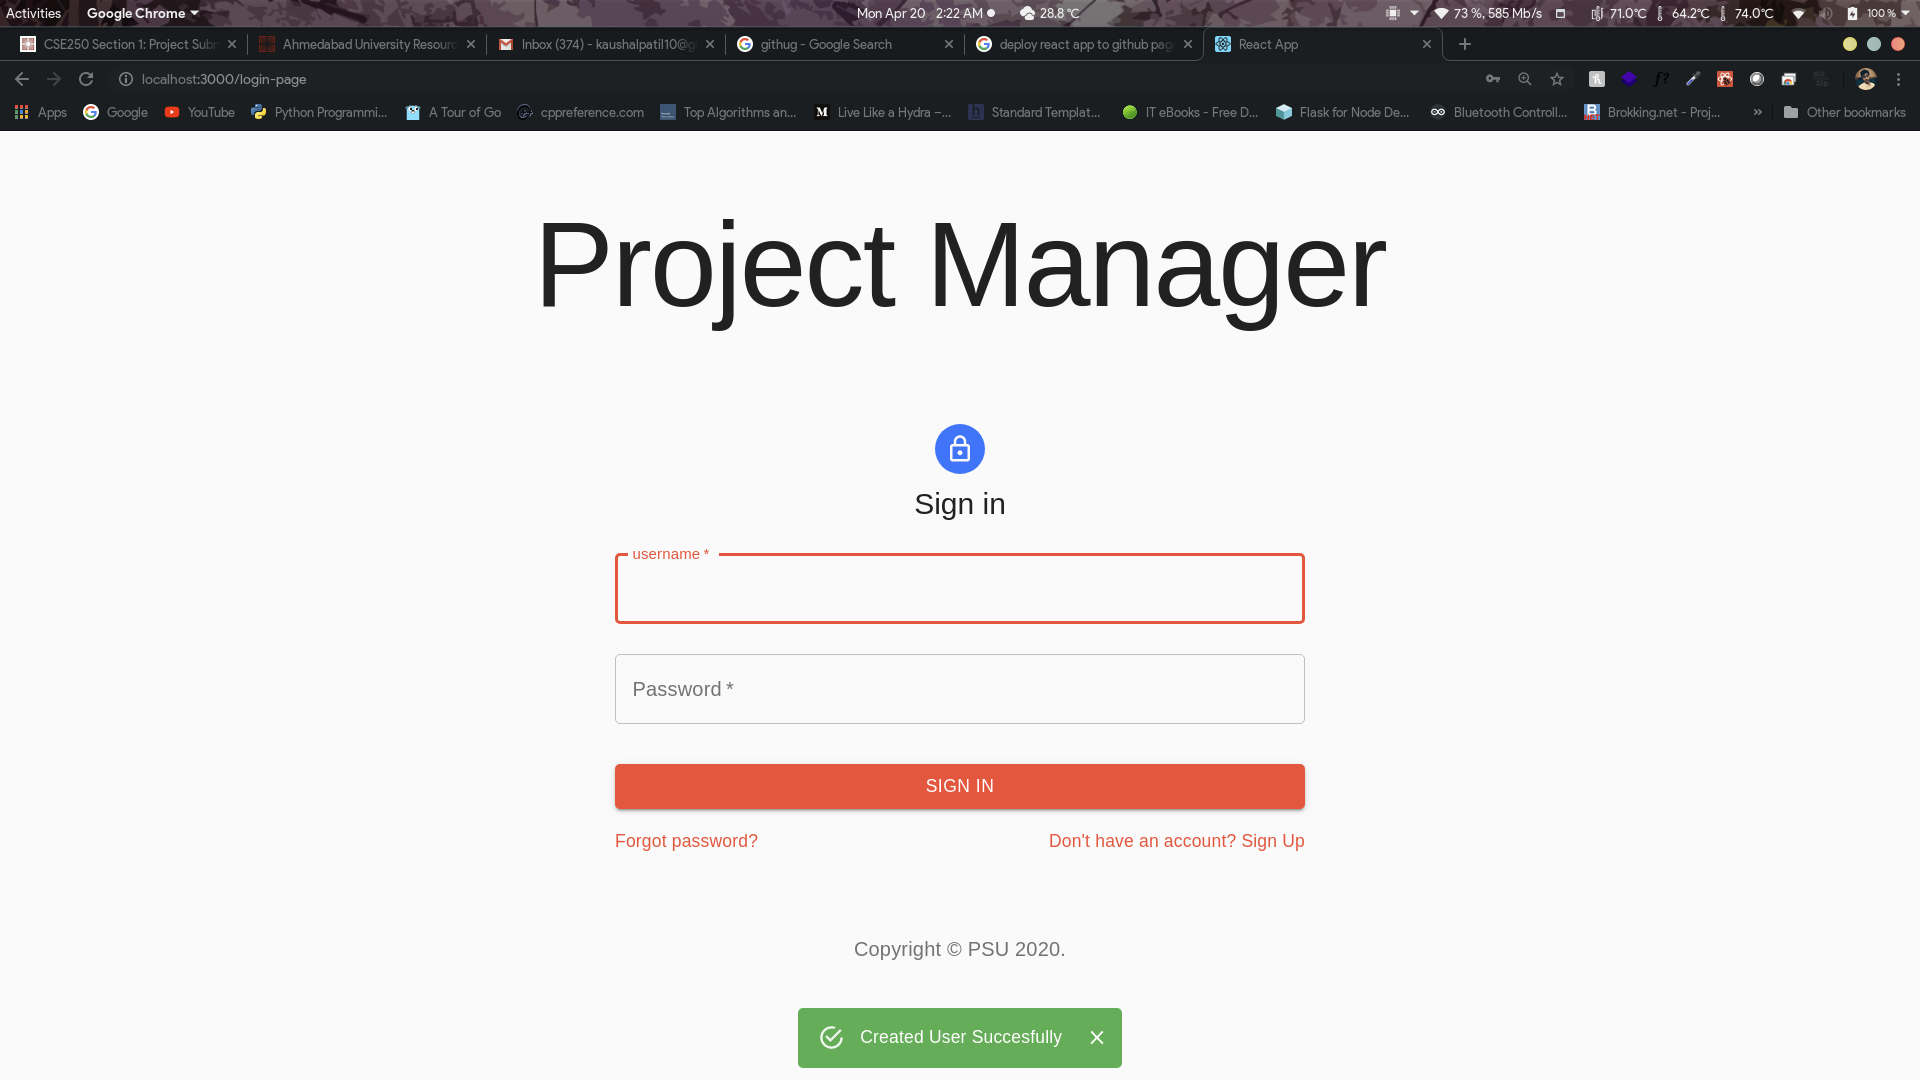
\includegraphics[scale=0.25]{./1.png}

Creation of board on adding projects and users

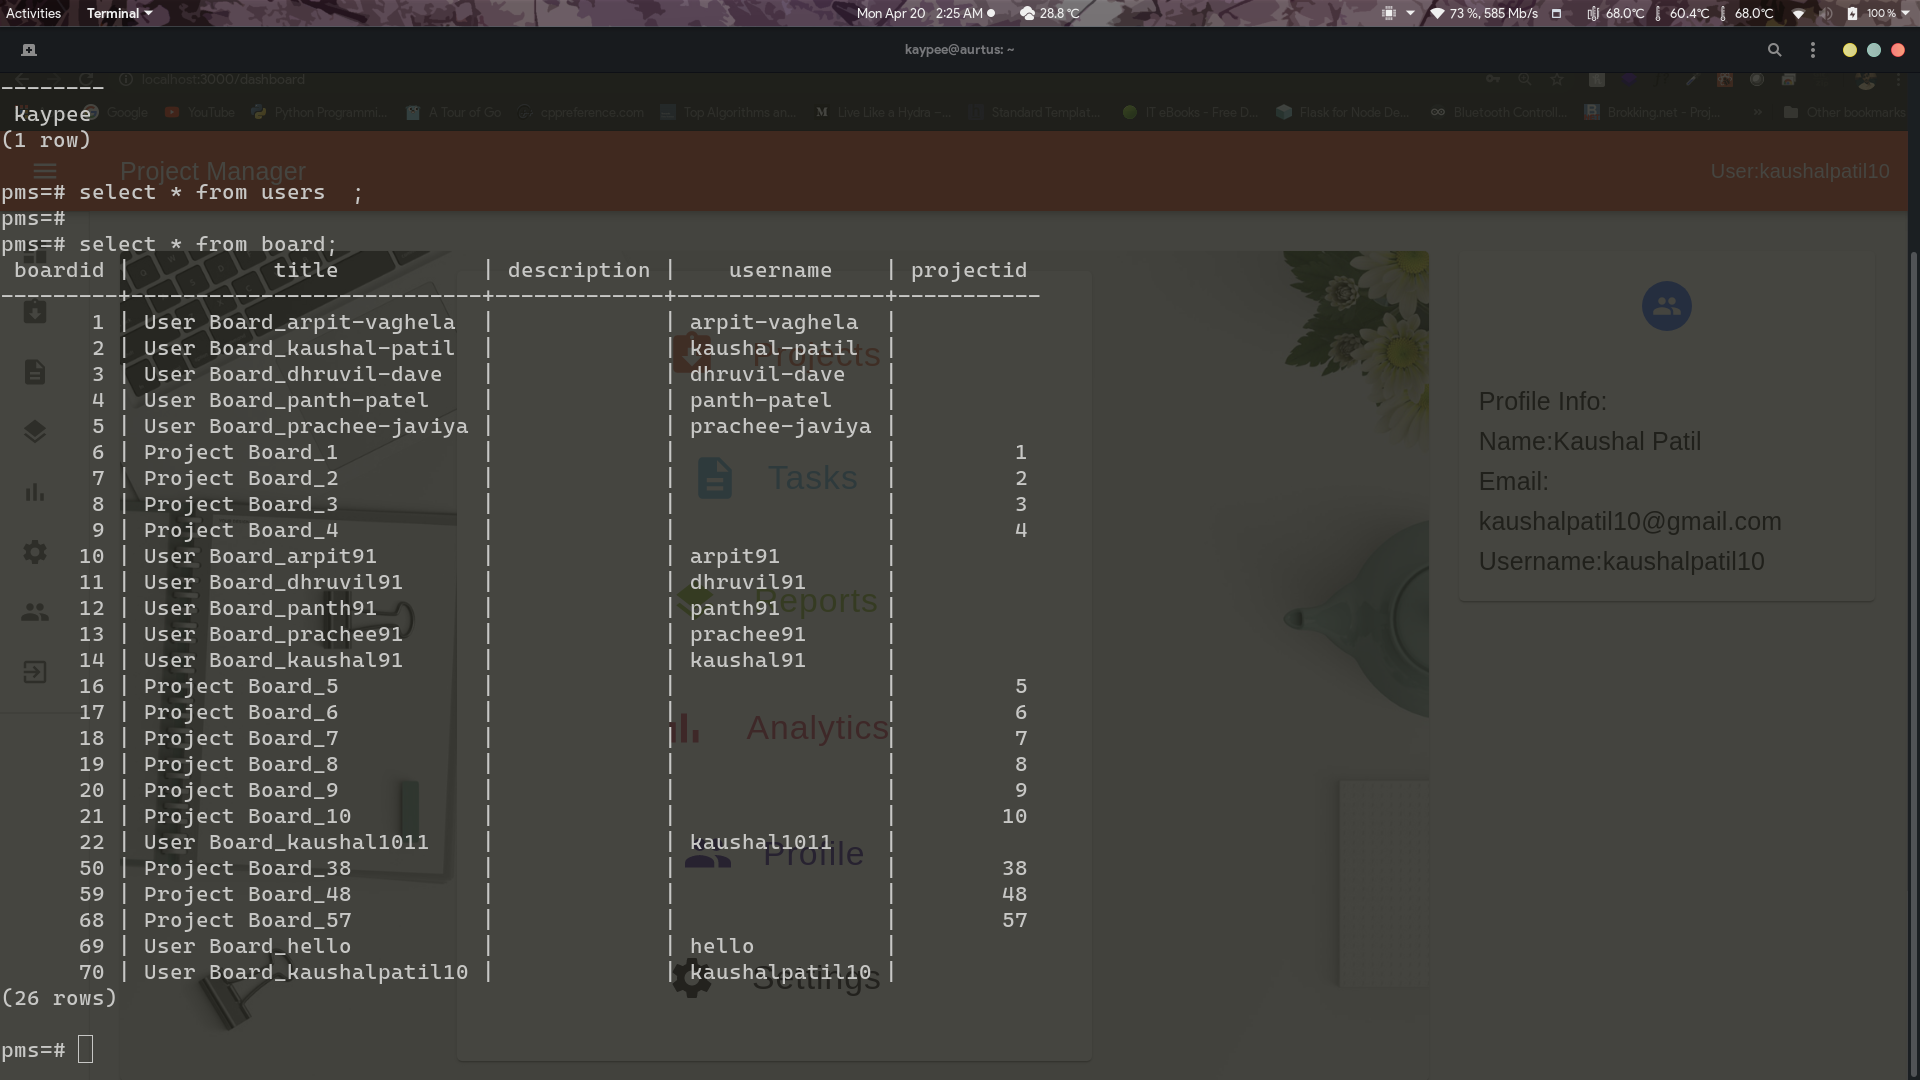
\includegraphics[scale=0.25]{./2.png}

Successful adding of tasks

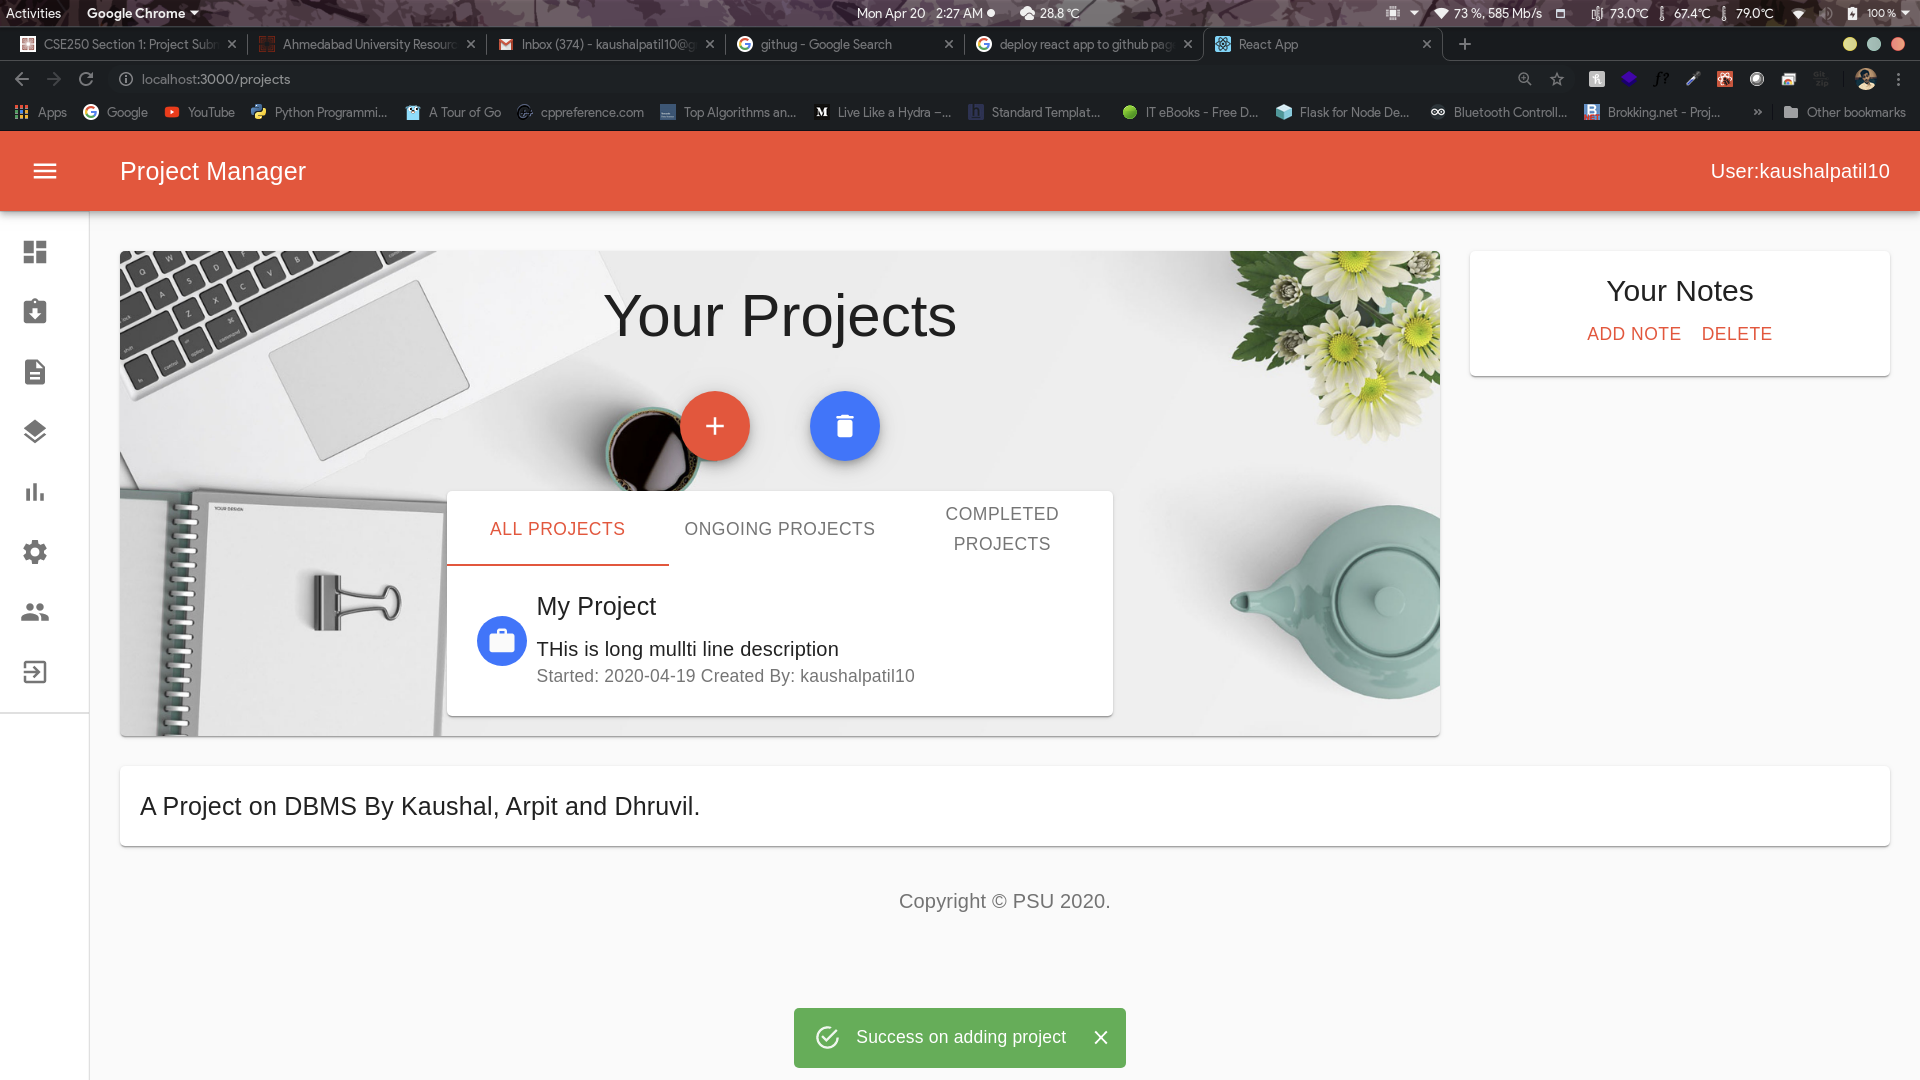
\includegraphics[scale=0.25]{./3.png}

Shows current users projects and files

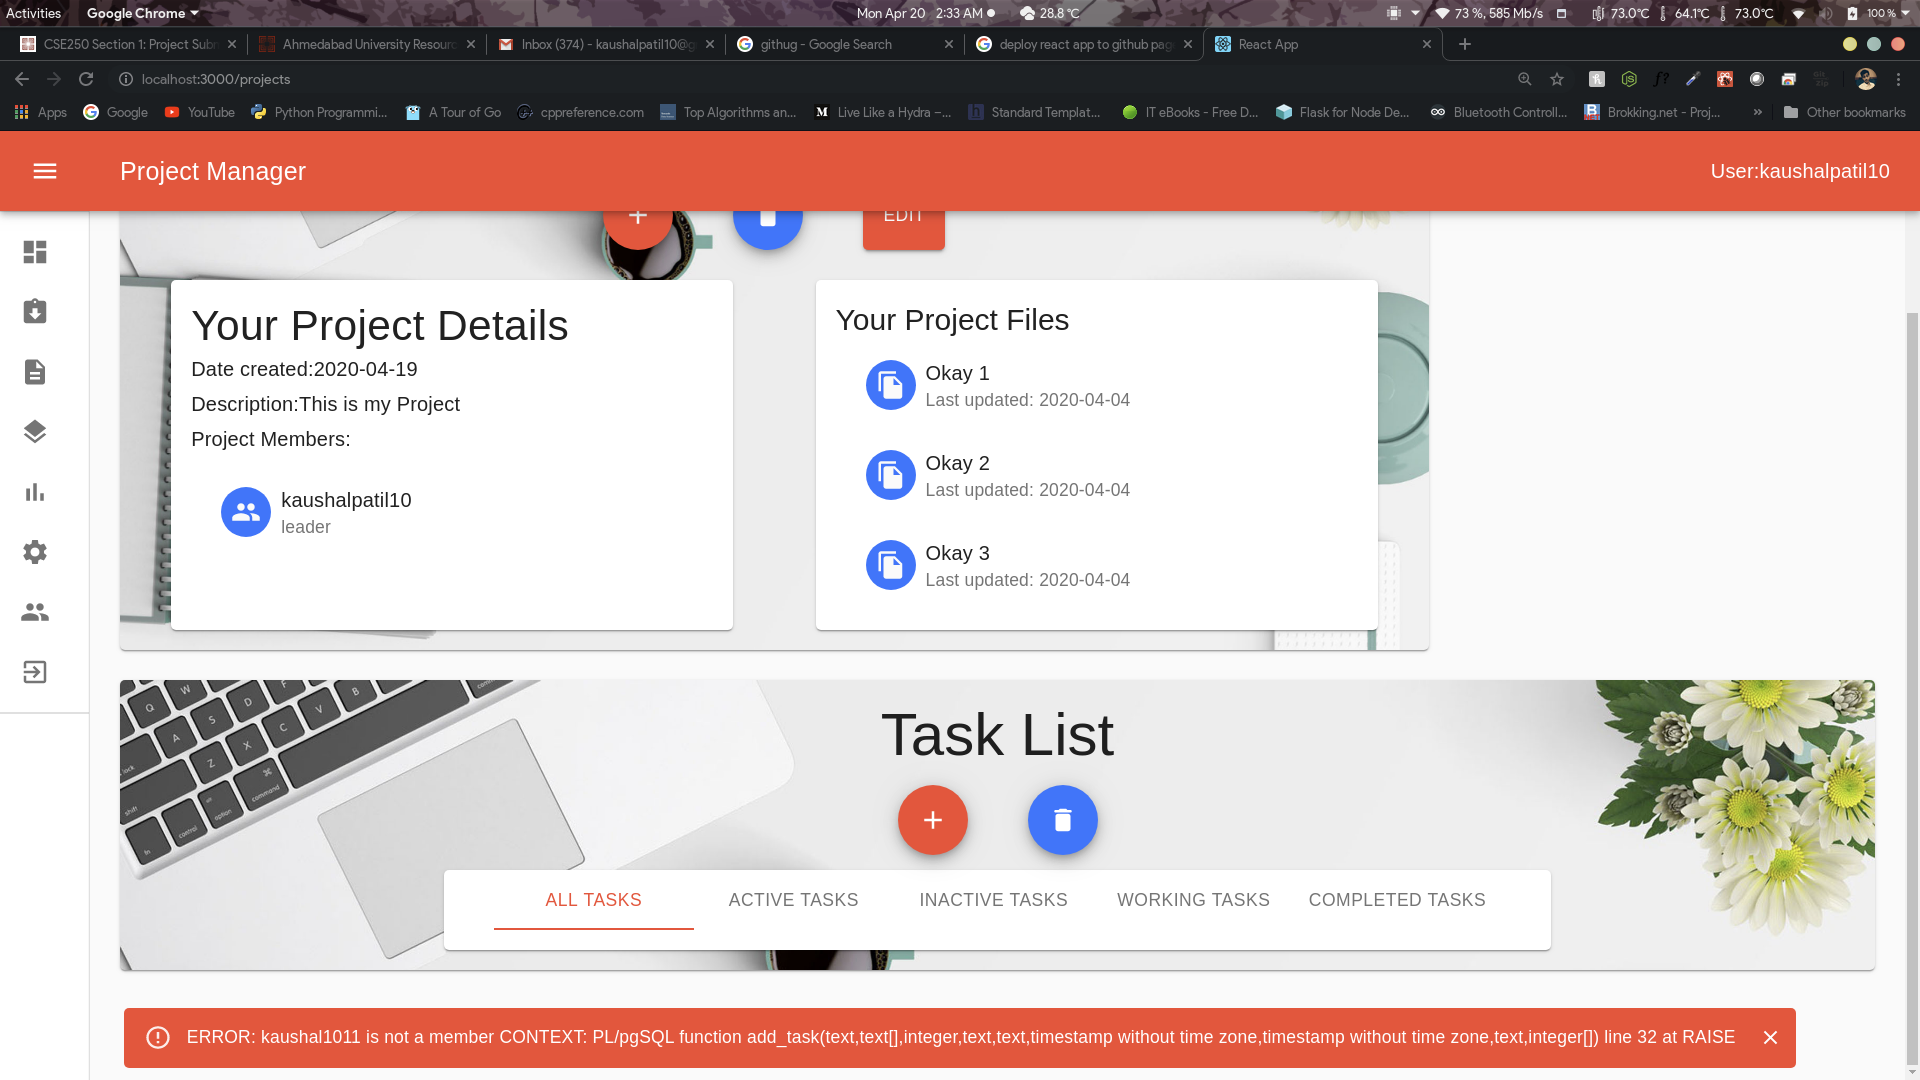
\includegraphics[scale=0.25]{./4.png}

Image

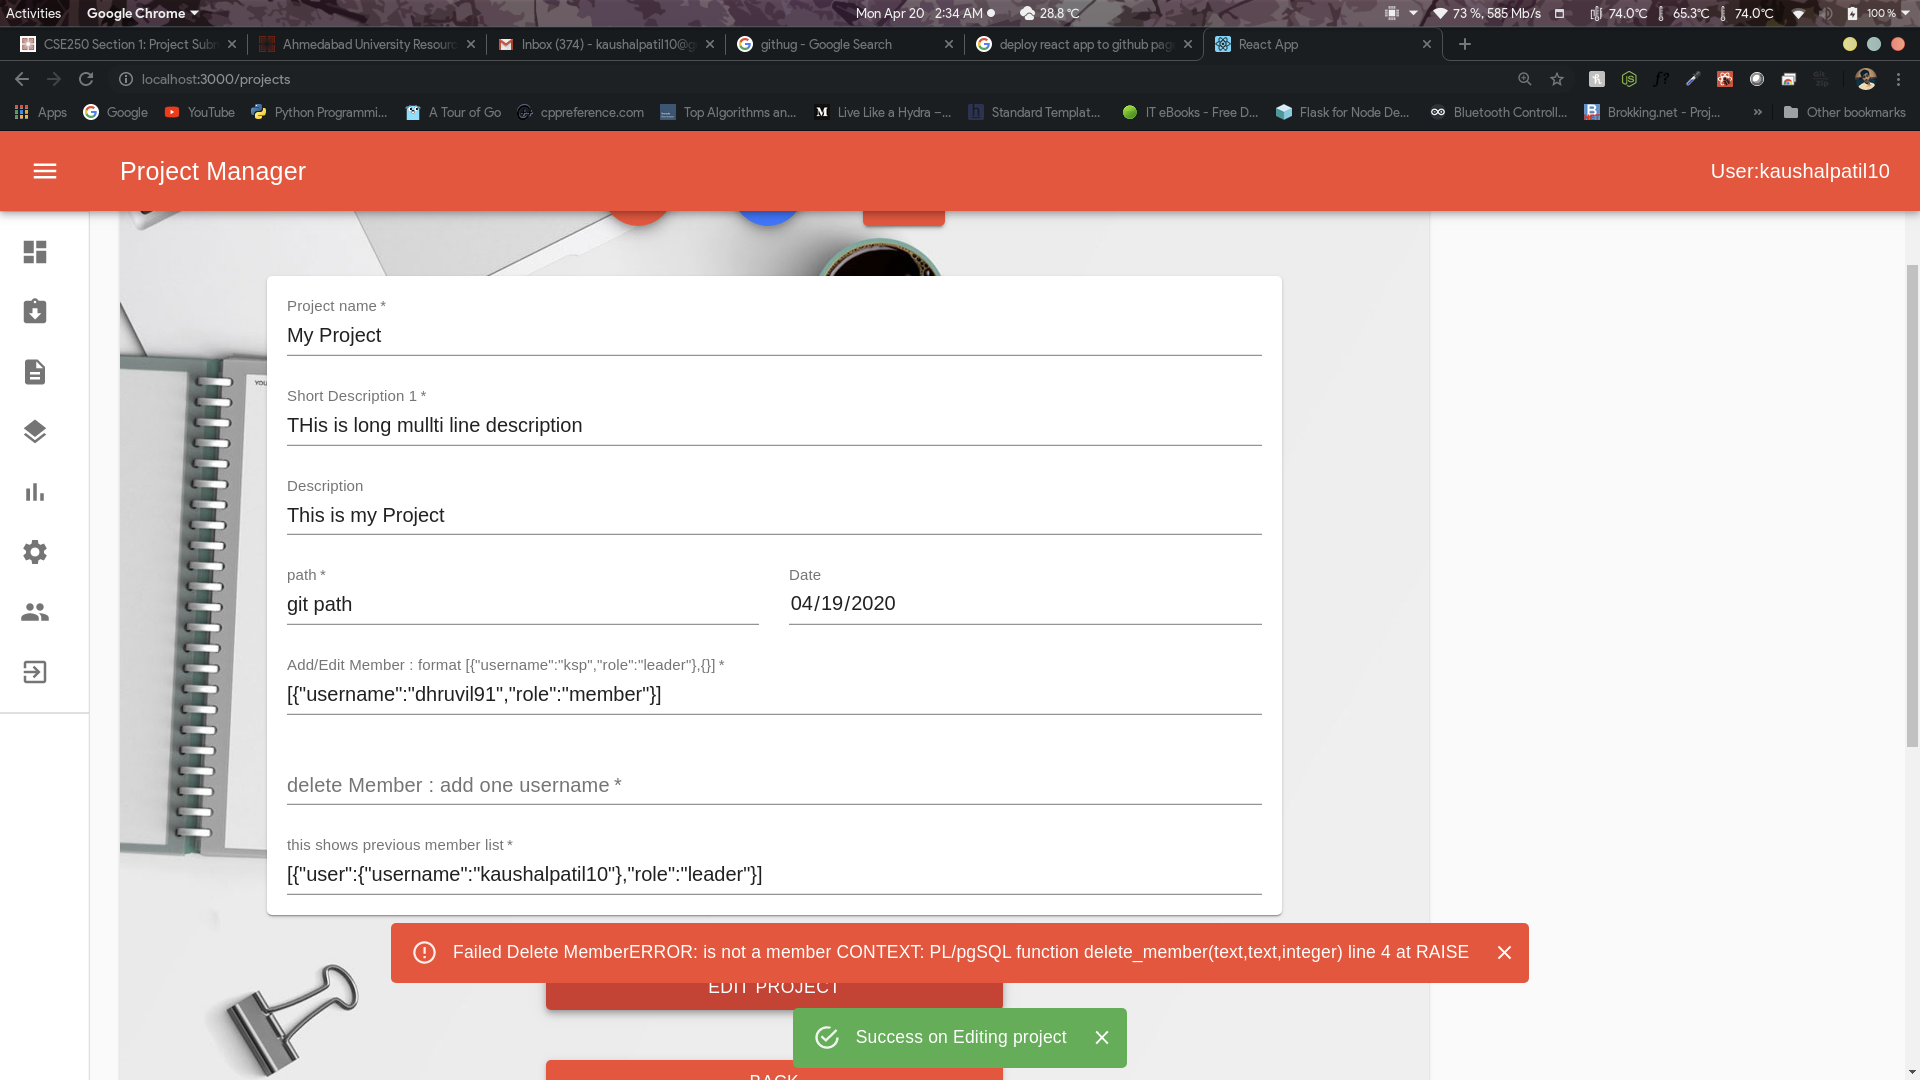
\includegraphics[scale=0.25]{./5.png}

Prevents changing tasks if not a leader

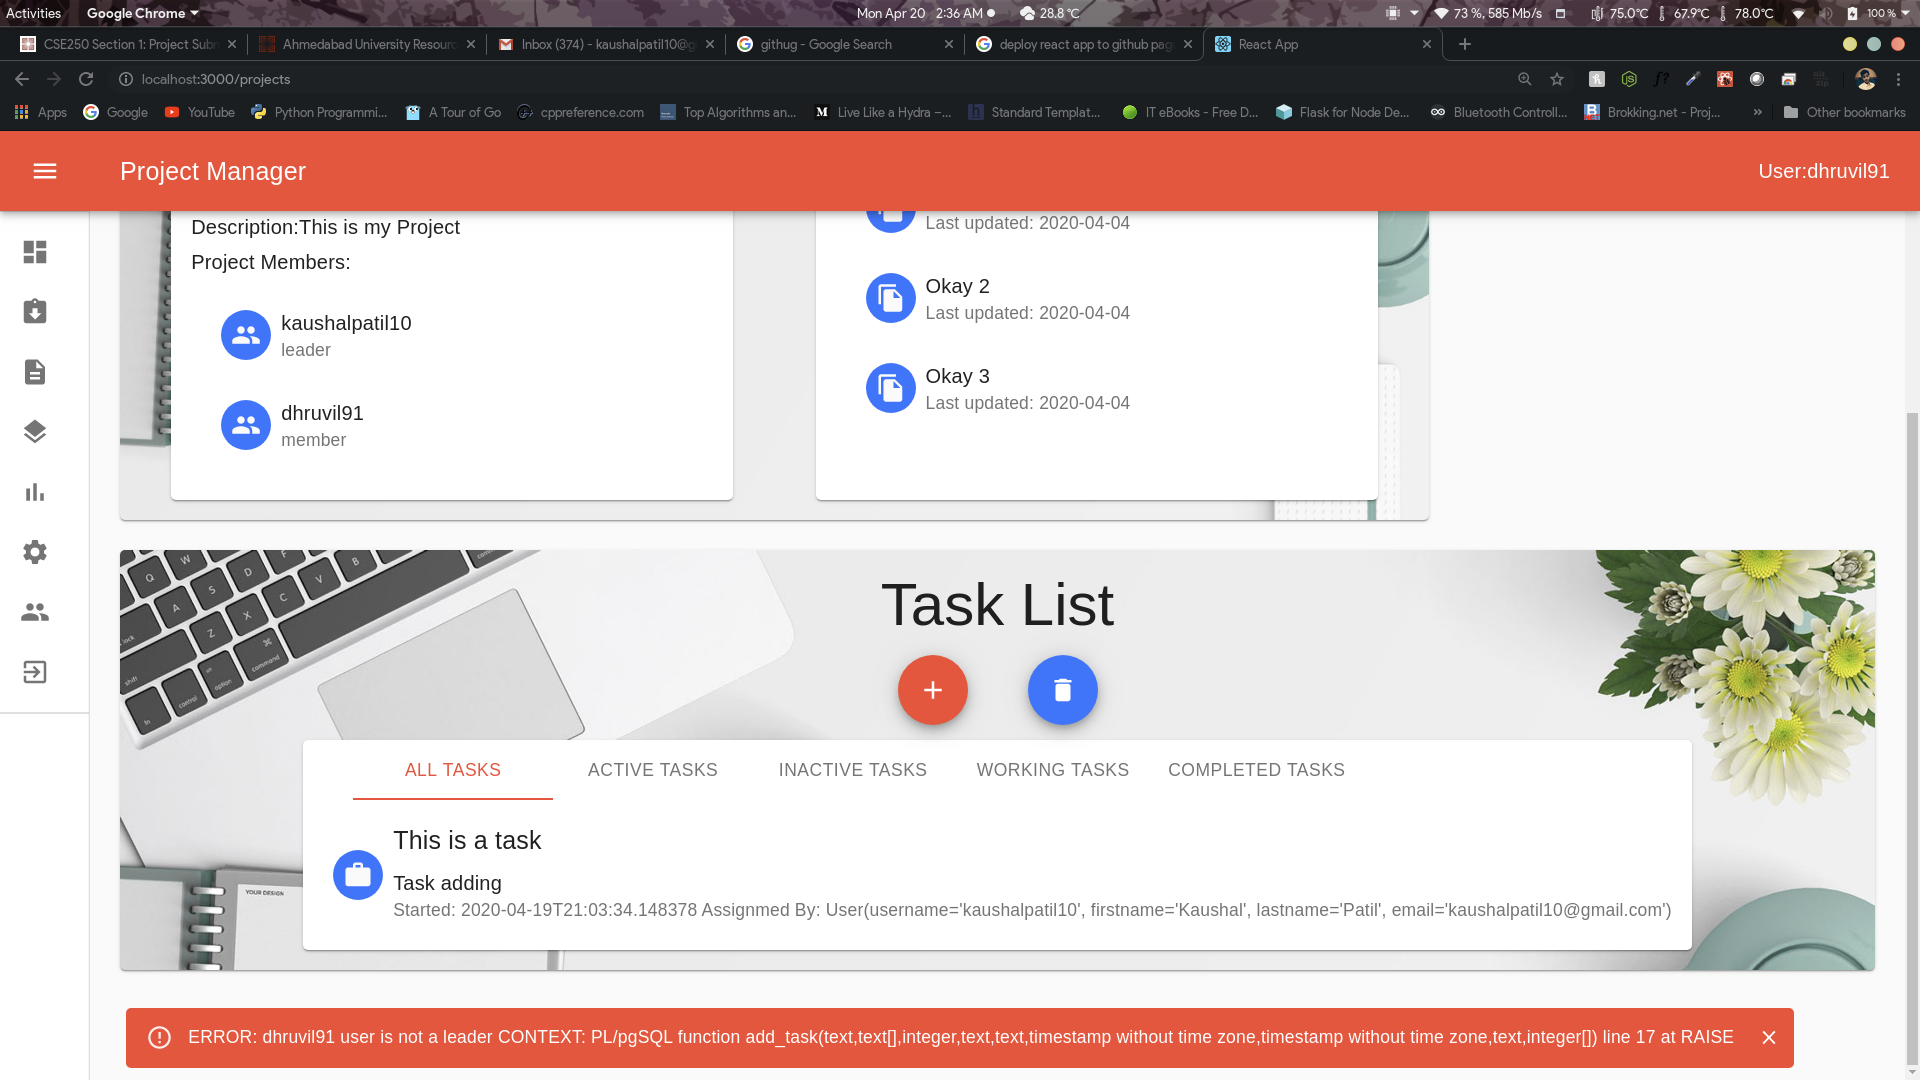
\includegraphics[scale=0.25]{./6.png}

\end{document}
